\documentclass{article}
\usepackage[utf8]{inputenc}
\usepackage[margin=0.8in]{geometry}

%\biboptions{sort&compress} %Change citations to be 1-10 if lots are listed

\usepackage{amsmath}
\usepackage{amsfonts} 
\usepackage{amssymb}
\usepackage{bm}
\usepackage{hyperref}

%For tables
\usepackage{booktabs}
\usepackage{multirow}
\usepackage{graphicx}

%For images
\graphicspath{{images/}}

%For subfigures
\usepackage{caption}
\usepackage{subcaption}

%For different coloured text
\usepackage{xcolor}

%For the bibliography
\usepackage[backend=biber,
			  style=ieee,
            sortcites=true,
            sorting=none]{biblatex}

%citestyle=numeric-comp,
%bibstyle=authoryear,       
\addbibresource{Bibliography.bib}

\title{MIL 780 - Assignment Two}
\author{Ryan Balshaw}
\date{05 April 2022}

\begin{document}

\maketitle

\section*{Foreword}
All code, documents and work relevant to this assignment can be found in my \href{https://github.com/RyanBalshaw/MIL_780_assignments}{\textcolor{blue}{Github repository}}.

\section{Question 1}

Consider the following model
\begin{equation}\label{eq:Q1_model}
x_n = \theta  + \epsilon_n,
\end{equation}
where $\epsilon_n \sim \mathcal{N}(0, \sigma^2)$. Given some observed data $\mathbf{x} = [x_1, \cdots, x_N]^T$, the objective is to perform Bayesian inference through a grid-based approach and a conjugate prior approach.


\subsection{Part A: Grid-based Bayesian inference}

Assume that $\sigma$ is known and given by $\sigma = 1.5$. Assume a Laplacian prior for $\theta$ with the following form:
\begin{equation}
 p(\theta) = L(\theta \vert 0, 2),
\end{equation}    
where 0 is the location parameter and 2 is the scaling parameter. A grid-based approach where $\theta \in [-10, 20]$ is used in the results to follow. There are a number of aspects that are of great important to Bayesian inference:
\begin{itemize}
\item The generative model $p(x \vert \theta)$.
\item The prior $p(\theta)$ over the generative model parameters.
\item The likelihood function $\mathcal{L}(\mathbf{x}, \theta)$.
\item The unnormalised posterior $p(\mathbf{x} \vert \theta)p(\theta)$.
\item The model evidence $p(\mathbf{x})$.
\item The posterior distribution $p(\theta \vert \mathbf{x})$.
\item The posterior predictive distribution $p(x \vert \mathbf{x})$.
\end{itemize}

In this part of the assignment, the objective is to gain exposure to each of these aspects for a simple one-dimensional problem.

\subsubsection{The prior distribution}
The prior over $\theta$ is given analytically as
\begin{equation}
p(\theta) = L(\mu, b) = \frac{1}{2b} e^{-\frac{\vert x - \mu \vert}{b}},
\end{equation}
and the logarithm of this distribution is equal to
\begin{equation}
\log p(\theta) = -\log ( 2\cdot b ) - \frac{\vert x - \mu \vert}{b}.
\end{equation}
In Figure \ref{fig:Q1a_prior} the prior and the log-prior is shown for $\mu = 0$ and $b = 2$. 
\begin{figure}[htb!]
\centering
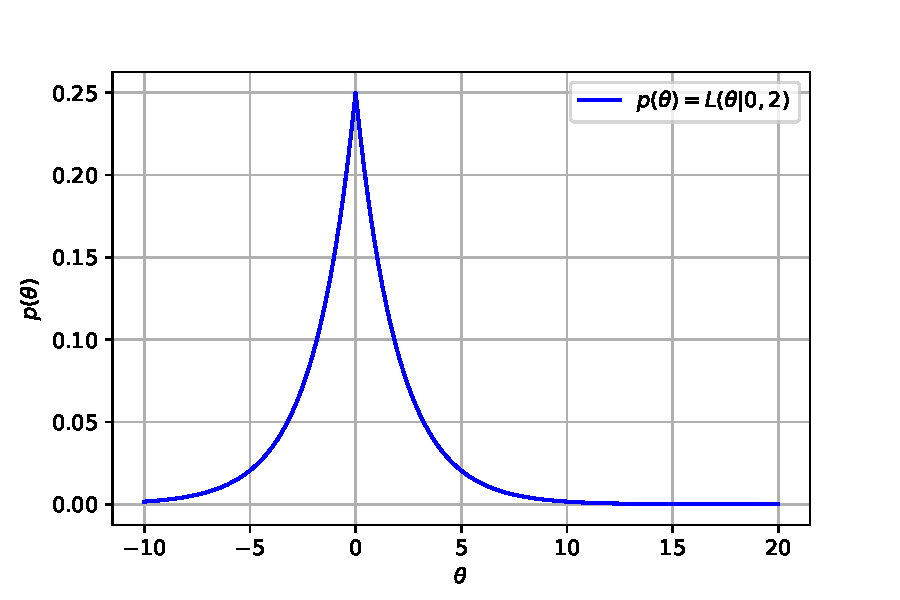
\includegraphics[scale=0.6]{Q1a_2.pdf}
\caption{The prior distribution function $p(\theta)$ visualised over the domain $\theta \in [-10, 20]$.}
\label{fig:Q1a_prior}
\end{figure}


\subsubsection{The generative model and the likelihood function}

Given the model in Equation \eqref{eq:Q1_model}, the model distribution over x is given as
\begin{equation}
\begin{aligned}[b]
p(x \vert \theta) &= \mathcal{N}(x \vert \theta, \sigma^2) \\
&= \frac{1}{\sqrt{2 \cdot \pi \cdot \sigma^2}} e^{-\frac{1}{2\sigma^2} \cdot \left( x - \theta \right)^2}.
\end{aligned}
\end{equation}
Given some observed data $\mathbf{x}$, where $\mathbf{x}$ is a column vector $\mathbf{x} \in \mathbb{R}^{N \times 1}$ and $N$ is the number of observed samples, the likelihood function, given $\theta$, is
\begin{equation}
\mathcal{L}(\mathbf{x}, \theta) = \prod_{n=1}^{N} p(x_n \vert \theta).
\end{equation}
The log-likelihood function may be given as
\begin{equation}
\begin{aligned}[b]
\mathcal{LL}(\mathbf{x}, \theta) &= \sum_{n=1}^{N} \log p(x_n \vert \theta) \\
&= \sum_{n=1}^{N} \left[ -\frac{1}{2}\log (2\cdot \pi) - \frac{1}{2}\log (\sigma^2) - \frac{\left( x - \theta \right)^2}{2\sigma^2} \right] \\
&= -\frac{N}{2}\log (2\cdot \pi) - \frac{N}{2}\log (\sigma^2) - \sum_{n=1}^{N} \left[\frac{\left( x - \theta \right)^2}{2\sigma^2} \right].
\end{aligned}
\end{equation}
It is important here to remind ourselves (read: myself) of the functions of the $\mathcal{LL}$ function. The observed data is typically fixed, and thus the only variable that we can alter is $\theta$. Thus, we can plot how the likelihood/log-likelihood function varies with $\theta$. In Figure \ref{fig:Q1a_likelihood} the likelihood function and log-likelihood function over $\theta$ is shown. Furthermore, the likelihood function is the joint probability of the observed data given the model parameters. In Bayesian inference, the likelihood function is key to finding the posterior distribution $p(\theta \vert \mathbf{x})$.
\begin{figure}[htb!]
\centering
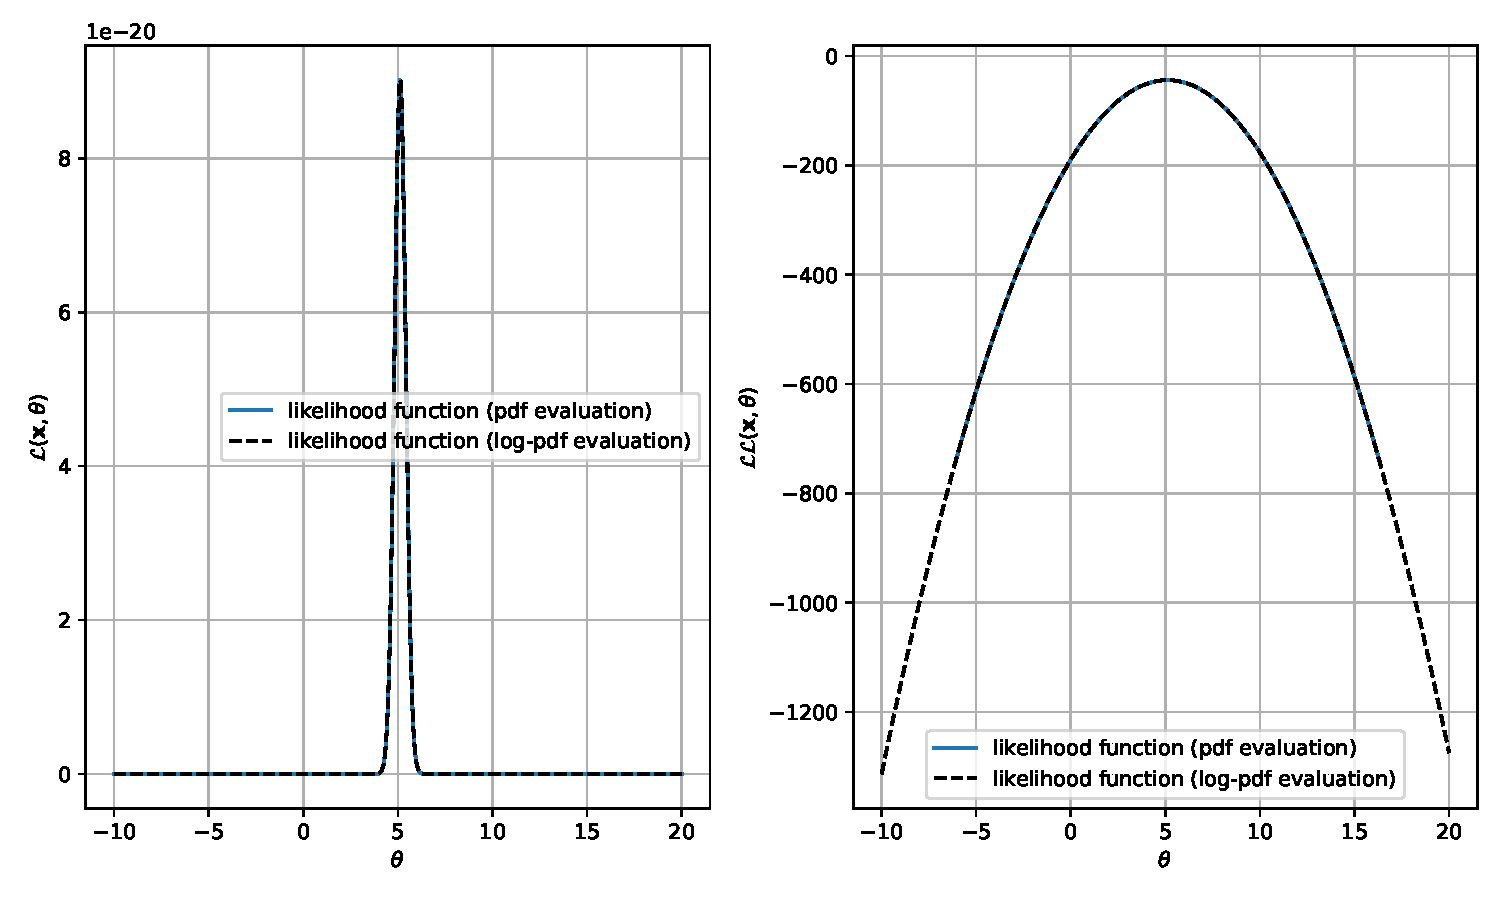
\includegraphics[scale=0.6]{Q1a_3.pdf}
\caption{The likelihood function $\mathcal{L}(\mathbf{x}, \theta)$ of the generative model $p(x \vert \theta)$ over the domain $\theta \in [-10, 20]$. In a) the likelihood function is shown, and in b) the log-likelihood function is shown.}
\label{fig:Q1a_likelihood}
\end{figure}

\subsubsection{The unnormalised posterior}
The unnormalised posterior is the numerator of posterior distribution over $\theta$ given $\mathbf{x}$. The posterior is given through Bayes' rule
\begin{equation}\label{eq:Q1_Bayes}
p(\theta \vert \mathbf{x}) = \frac{p(\mathbf{x}\vert\theta)p(\theta)}{p(\mathbf{x})}.
\end{equation}
It is now clear why the prior was the first step of the Bayesian process. We assume a prior over $\theta$, observe some data $\mathbf{x}$ and then we can inspect the posterior $p(\theta \vert \mathbf{x})$. To do this, we need the unnormalised posterior $p(\mathbf{x}\vert\theta)p(\theta)$ and the model evidence $p(\mathbf{x})$. To determine the unnormalised posterior we can use the analytical forms of the likelihood function and the prior distribution
\begin{equation}
\begin{aligned}[b]
p(\mathbf{x}, \theta) &= p(\mathbf{x}\vert\theta)p(\theta) \\
\mathcal{F}(\theta, \mathbf{x}, , \sigma, \mu_\theta, b) &= \frac{1}{2 \cdot b} \exp{ \left(- \frac{\vert \theta - \mu_\theta \vert}{b} \right)} \prod_{n=1}^{N} \frac{1}{ \sqrt{2 \cdot \pi \cdot \sigma^2}} \exp{ \left(-\frac{1}{2\sigma^2} \cdot \left( x_n - \theta \right)^2 \right)},
\end{aligned}
\end{equation}
where $\mathcal{F}(\theta, \mathbf{x}, \sigma, \mu_\theta, b)$ is the notation that I have adopted to show the parameters of the unnormalised posterior. In this case, $\sigma$, $\mu_\theta$ an $b$ are fixed to $\sigma =1.5$,  $\mu_\theta = 0$ and $b = 2$. It is also possible to inspect the log-unnormalised posterior, and this is given analytically as
\begin{equation}
\begin{aligned}[b]
\log p(\mathbf{x}, \theta) &= \log p(\mathbf{x}\vert\theta) + \log p(\theta) \\
\mathcal{LF}(\theta, \mathbf{x}, , \sigma, \mu_\theta, b) &= \sum_{n=1}^{N} \left[ -\frac{1}{2}\cdot\log (2\cdot \pi) - \frac{1}{2}\cdot\log (\sigma^2) - \frac{\left( x_n - \theta \right)^2}{2\sigma^2} \right]  -\log ( 2\cdot b ) - \frac{\vert \theta - \mu_\theta \vert}{b} \\ 
&= -\frac{N}{2} \cdot \log (2\cdot \pi) - \frac{N}{2} \cdot \log (\sigma^2) - \log ( 2\cdot b ) - \frac{\vert \theta - \mu_\theta \vert}{b} - \sum_{n=1}^{N} \frac{\left( x_n - \theta \right)^2}{2\sigma^2}.
\end{aligned}
\end{equation}
In Figure \ref{fig:Q1a_unnorm_posterior} the unnormalised posterior is shown. Notice how the prior and likelihood function influences the unnormalised posterior. There appears to be a slight shift towards the origin, and the influence of the prior is marginal in comparison to the likelihood function. The marginal influence of the prior is attributed to the prior parameters, as the prior is far from the likelihood function and the variance ensures that the prior is numerically larger over the $\theta$ domain in comparison to the likelihood function. Decreasing the variance or shifting the prior mean should increase its influence on the unnormalised posterior.  
\begin{figure}[htb!]
\centering
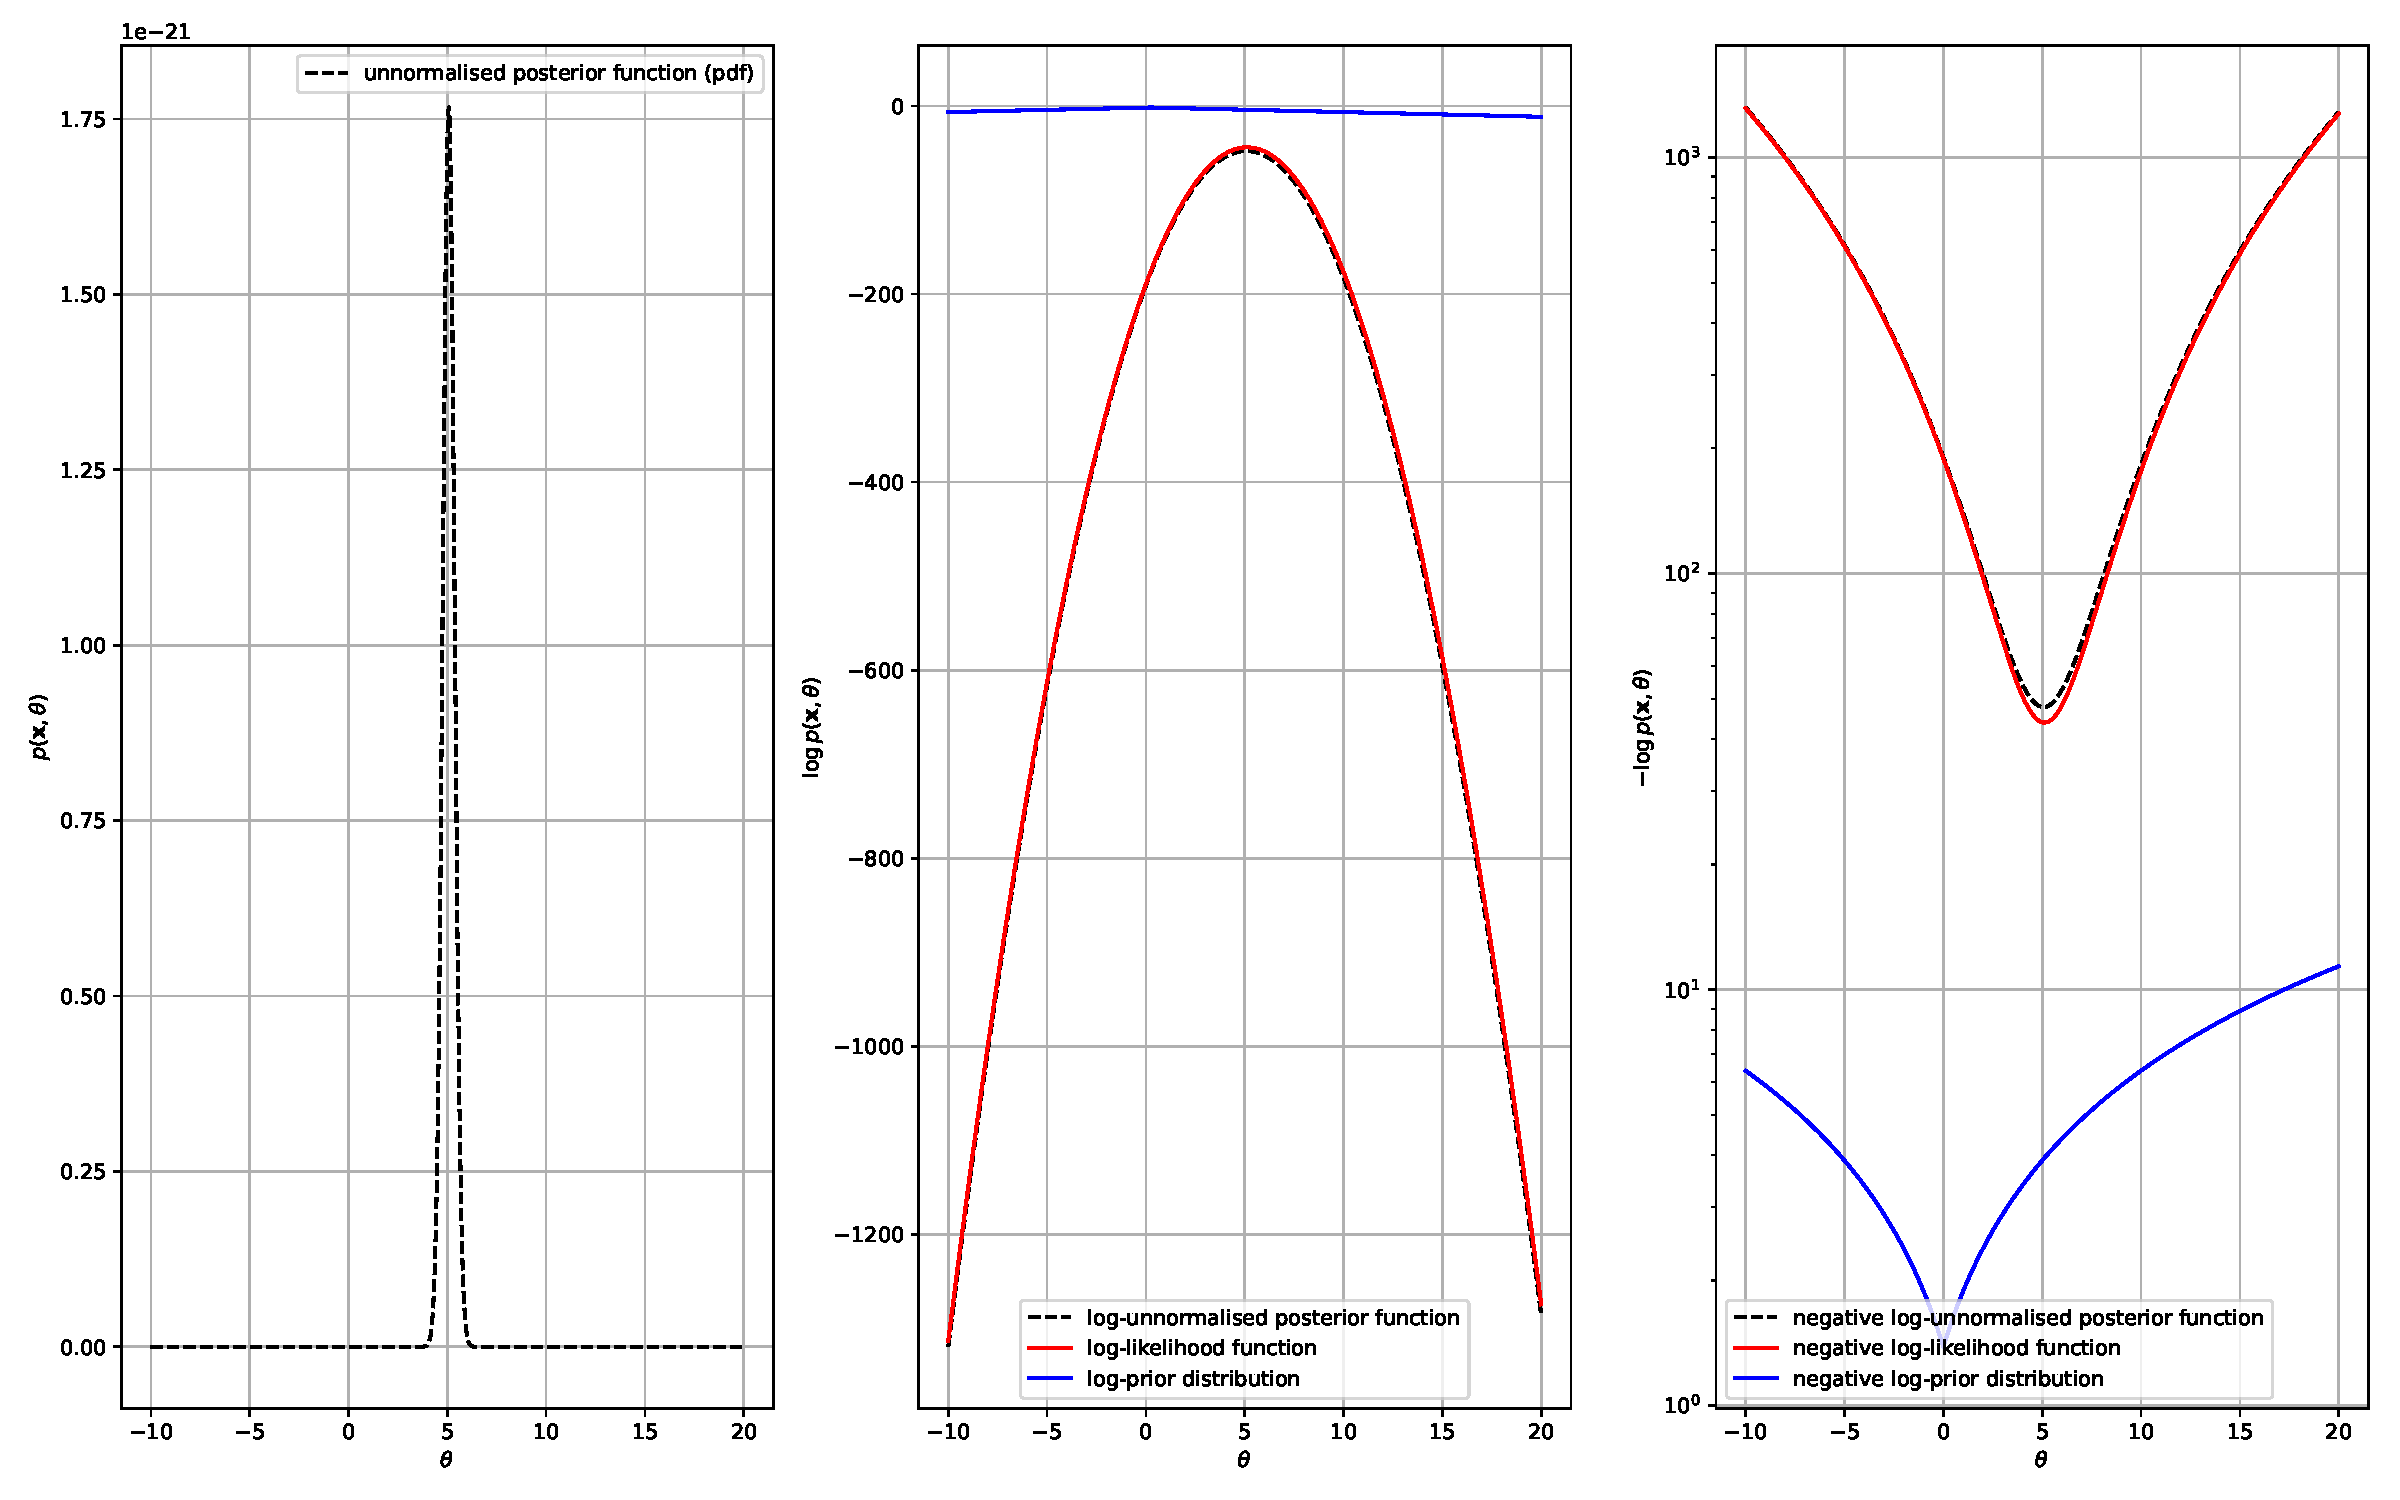
\includegraphics[scale=0.4]{Q1a_4.pdf}
\caption{The unnormalised posterior distribution $\mathcal{F}(\theta, \mathbf{x}, \sigma, \mu_\theta, b)$ for $\sigma  =1.5, \mu_\theta = 0$ and $b = 2$ over the domain $\theta \in [-10, 20]$. Three variations of the unnormalised posterior is visualised here, the standard unnormalised posterior, the logarithm of the unnormalised posterior and the terms therein, and the negative of the unnormalised log-posterior.}
\label{fig:Q1a_unnorm_posterior}
\end{figure}

\subsubsection{The model evidence}
In order to determine the posterior distribution over the parameters $p(\theta \vert \mathbf{x})$, we need to determine the denominator of Equation \eqref{eq:Q1_Bayes}. The denominator is commonly referred to as the model evidence, and it is sometimes known as the marginal likelihood $p(\mathbf{x})$. Note that this marginalisation is with respect to the generative model parameters and represents the probability of the observed data marginalized over the parameters $\theta$. This is given formally as
\begin{equation}
\begin{aligned}[b]
p(\mathbf{x}) &= \int_\theta p(\mathbf{x}, \theta) d\theta \\
&= \int_\theta p(\mathbf{x} \vert \theta) p(\theta) d\theta \\
&= 1.32856e^{-21}.
\end{aligned}
\end{equation}

\subsubsection{The posterior distribution}
Now that we know the model evidence, we can use the unnormalised posterior and normalise it by the model evidence to obain the posterior distribution $p(\theta \vert \mathbf{x})$. In Figure \ref{fig:Q1a_posterior} the posterior distribution for the model parameter $\theta$ is shown. Notice how the model evidence, which is a constant, effectively rescales the unnormalised posterior. This is to ensure that the posterior distribution is a true distribution (i.e., it satisfies $\int_\theta p(\theta \vert \mathbf{x})d\theta = 1$ and $p(\theta \vert \mathbf{x}) > 0$  $\forall$  $\theta$).
\begin{figure}[htb!]
\centering
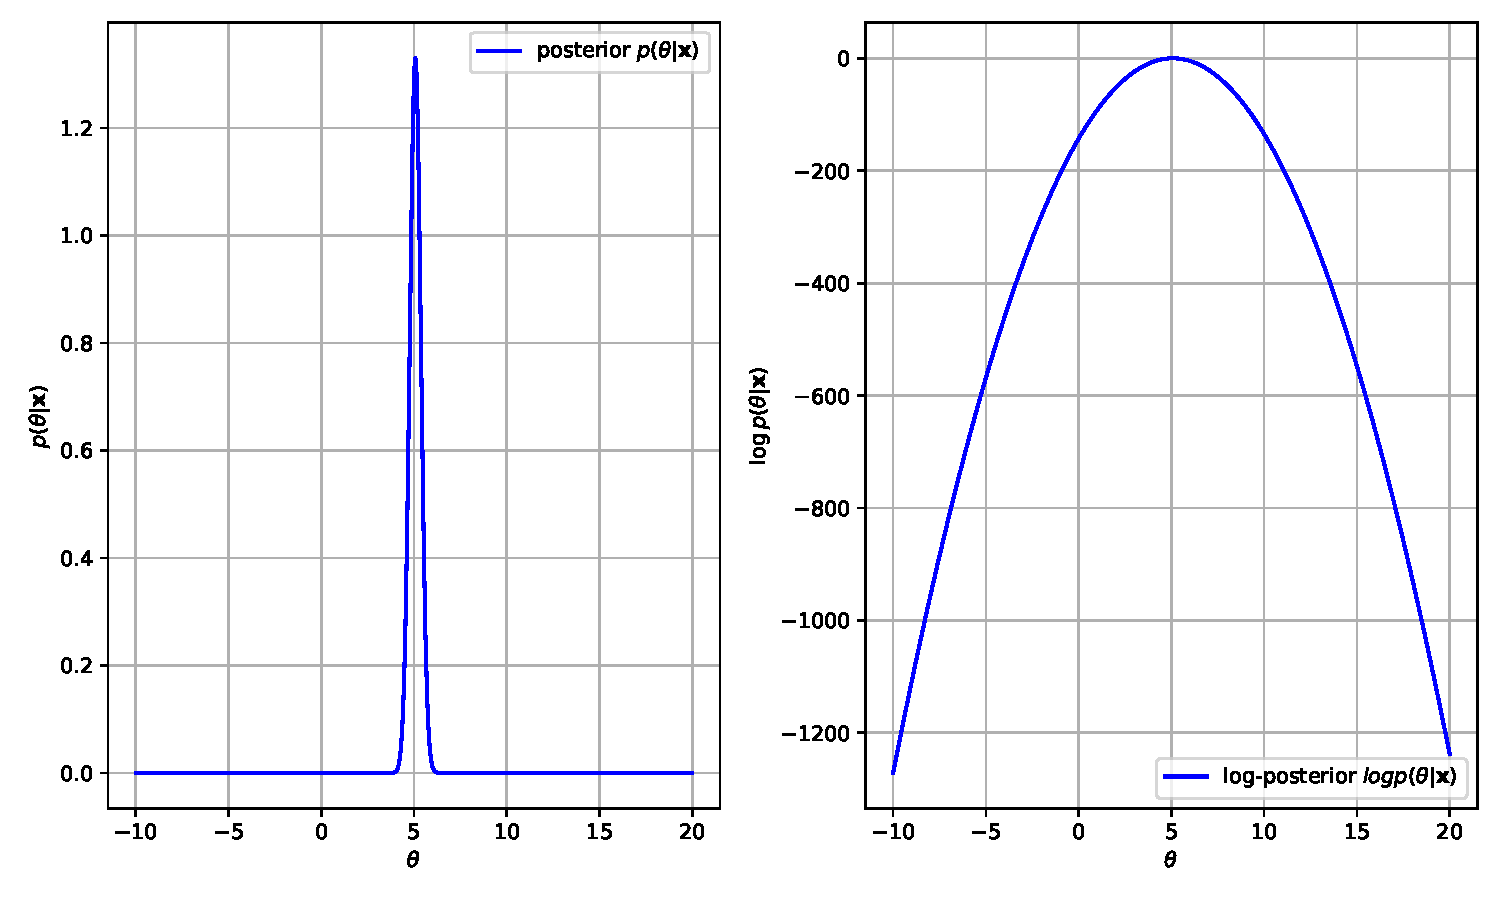
\includegraphics[scale=0.6]{Q1a_5.pdf}
\caption{The posterior distribution $p(\theta \vert \mathbf{x})$ and the logarithm thereof over the domain $\theta \in [-10, 20]$. The MAP solution is given in Table \ref{tab:Q1_a}.}
\label{fig:Q1a_posterior}
\end{figure}

\subsubsection{The posterior predictive distribution}
However, finding the posterior distribution is only only part of the Bayesian inference puzzle. We would still like to use the generative model given in Equation \eqref{eq:Q1_model} for any newly observed data and to do so, we need to incorporate the posterior distribution in some way. A naive, but viable approach is to use the maximum-a-posteriori (MAP) estimate from the unnormalised posterior as a basis for the model parameter $\theta$. However, this is simply a parameter re-substitution of the estimator for $\theta$ and is equivalent to maximum likelihood estimation. The power of Bayesian inference is that we can incorporate all uncertainty in the unknown parameter when observing new data. This allows us to quantify new data under all possible variations of the unknown model parameter $\theta$ rather than on a maximum estimate\footnote{I found the following \href{https://stats.stackexchange.com/questions/242082/posterior-predictive-distribution-vs-map-estimate}{\textcolor{blue}{StackExchange}} discussion very insightful.}. To use the uncertainty of the unknown parameter for newly observed data, we can use the posterior predictive distribution. This is given as 
\begin{equation}\label{eq:Q1a_posterior}
p(x\vert \mathbf{x}) = \int_\theta p(x \vert \theta) p(\theta \vert \mathbf{x}) d\theta.
\end{equation}
In Figure \ref{fig:Q1a_posterior_predictive} the posterior predictive distribution is shown. In my implementation I used two methods to numerically estimate the integral in Equation \eqref{eq:Q1a_posterior}. The expensive version, where I used \texttt{scipy.integrate.quad}, took 202.154 seconds to perform 1000 iterations over $x$. The cheap version, where I used \texttt{scipy.integrate.trapz}, took 0.039 seconds to perform 1000 iterations over $x$. 
\begin{figure}[htb!]
\centering
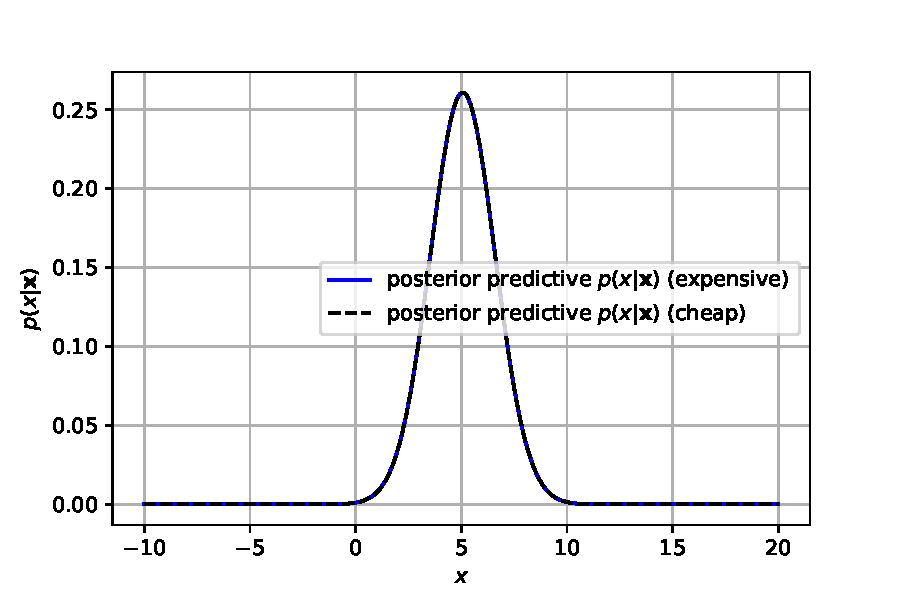
\includegraphics[scale=0.6]{Q1a_6.pdf}
\caption{The posterior predictive distribution $p(x \vert \mathbf{x})$ determined using a cheap and expensive computational methodology over the domain $\theta \in [-10, 20]$.}
\label{fig:Q1a_posterior_predictive}
\end{figure}

\subsubsection{Estimating estimators}
We can now compare different estimators for the unknown parameter $\theta$ using the prior distribution, the likelihood function and the unnormalised posterior function. This estimator estimation process can be performed using a grid-based approach, analytical solutions and through numerical optimisation techniques. In Table \ref{tab:Q1_a} the estimates for these three approaches is given. Notice how the MAP estimate is lower than the maximum likelihood (ML) estimate, which is due to the influence of the prior $p(\theta)$.
\begin{table}[htb!]
\centering
\caption{The estimates for the unknown parameter $\theta$ using the prior, maximum likelihood and maximum a posteriori. These estimates are found using a grid-based approach, analytically an using numerical optimisation.}
\label{tab:Q1_a}
\begin{tabular}{@{}cccc@{}}
\toprule
Approach & Prior & ML & MAP \\ \midrule
Grid-based & 0.0 & 5.1051 & 5.075 \\
Analytical & -0.0002 & 5.1161 & N/A \\
Numerical & 0.002737 & 5.1161 & 5.071 \\ \bottomrule
\end{tabular}
\end{table}

\subsubsection{Using Bayesian inference}
We can use the posterior distribution $p(\theta \vert \mathbf{x})$ and the posterior predictive distribution $p(x \vert \mathbf{x})$ to determine probabilities $p(a \leq X \leq b)$. The first probability of interest is $p(\theta \leq 4 \vert \mathbf{x})$ and the second is $p(x \leq 4 \vert \mathbf{x})$. As a reminded, the probability $p(a \leq x \leq b)$ may be given as
\begin{equation}
p(a \leq x \leq b) = F_x(b) - F_x(a),
\end{equation}
where $F_x(X) = \int_{-\infty}^{X} p(x) dx$ is the cumulative distribution function (CDF) of $p(x)$. As we do not know the analytical forms of the posterior and posterior predictive distributions, we cannot use an analytical expression for the CDFs. However, we have a discretised set of likelihoods along the $\theta$ and $x$ domain and thus we can estimate the CDF by cumulatively adding the likelihoods. It is assumed here that the CDF varies linearly between points along each respective domains. A linear interpolation approach is then used to estimate $F_x(X)$. This process ensures that we can estimate the probabilities of interest.

Using this approach, it was found that $p(\theta \leq 4 \vert \mathbf{x}) = 0.0002$ and $p(x \leq 4 \vert \mathbf{x}) = 0.2419$. In Figure \ref{fig:Q1a_CDFs} the CDFs of interest and the resulting probabilities are shown. The posterior probability that $\theta \leq 4$ informs us that it is very unlikely that a model parameter $\theta$ in this range is responsible for generating the observed data. The posterior predictive probability that $x \leq 4$ is noticeably larger, and this indicates that it is far more probable that newly observed $x$ samples may be drawn in the $x$ domain $x \in [-\infty, 4]$. 
\begin{figure}
     \centering
     \begin{subfigure}[b]{0.45\textwidth}
         \centering
         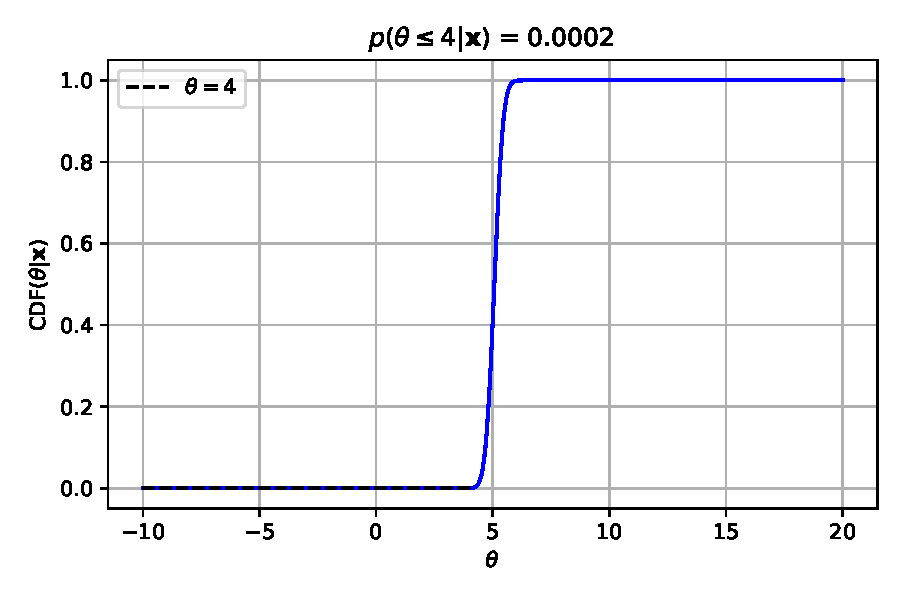
\includegraphics[width=\textwidth]{Q1a_7a.pdf}
         \caption{$F_{\theta \vert \mathbf{x}}(\theta)$.}
     \end{subfigure}
     ~
     \begin{subfigure}[b]{0.45\textwidth}
         \centering
         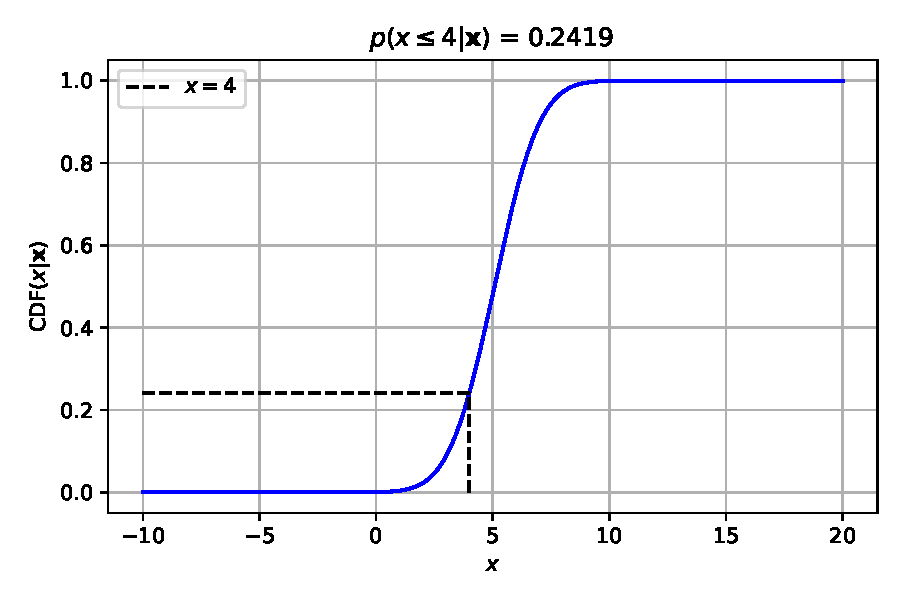
\includegraphics[width=\textwidth]{Q1a_7b.pdf}
         \caption{$F_{x \vert \mathbf{x}}(x)$.}
     \end{subfigure}
     
     \caption{The CDFs used to determine the probabilities $p(\theta \leq 4 \vert \mathbf{x})$ and $p(x \leq 4 \vert \mathbf{x})$ over the domain $\theta \in [-10, 20]$. In a) the CDF of the posterior distribution $p(\theta \vert \mathbf{x})$ is shown, while in b) the CDF of the posterior predictive distribution $p(x \vert \mathbf{x})$ is shown.}
     \label{fig:Q1a_CDFs}
\end{figure}

\subsubsection{Prior hyper-parameters}
At this point in the assignment we have assumed that the prior parameters are fixed in nature. However, there are no set values that are always given to these parameters. As such, all of the distributions of interest in Bayesian inference are conditioned on these parameters. Changing the mean of the prior distribution may be a biased procedure as we are effectively biasing the model towards a certain direction. While this is not always a bad decision, we can also control the impact of the prior in the Bayesian inference process using the prior variance. The prior is parametrised as 
\begin{equation}
p(\theta; \alpha) = L(\theta \vert 0, \alpha)
\end{equation}
where $\alpha$ is a hyper-parameter. The prior hyper-parameter is noticeably influential in posterior distribution
\begin{equation}
p(\theta \vert \mathbf{x}, \alpha) = \frac{p(\mathbf{x}\vert \theta)p(\theta \vert \alpha)}{p(\mathbf{x} \vert \alpha)},
\end{equation}
and the model evidence
\begin{equation}
\begin{aligned}[b]
p(\mathbf{x}) &= \int_\theta p(\mathbf{x}, \theta) d\theta \\
&= \int_\theta p(\mathbf{x} \vert \theta) p(\theta \vert \alpha) d\theta.
\end{aligned}
\end{equation}
As such, a range of $\alpha$ values were considered and the effects on the posterior distribution, the MAP estimate and the model evidence were inspected. In Figure \ref{fig:Q1a_alpha_variation} the results of varying $\alpha$ is shown. It is clear from Figure \ref{fig:Q1a_alpha_variation}b) that by increasing the variance we approach a region where the MAP estimate steadies out. Furthermore, as seen in Figure \ref{fig:Q1a_alpha_variation}d) a larger variance produces a posterior distribution with smaller variation. It is clear that small model variances strongly affect the Bayesian inference process. This implies that having a `tight' prior increases its influence in the results, whereas a prior with a larger variance decreases its influence.
\begin{figure}[htb!]
     \centering
     \begin{subfigure}[b]{0.45\textwidth}
         \centering
         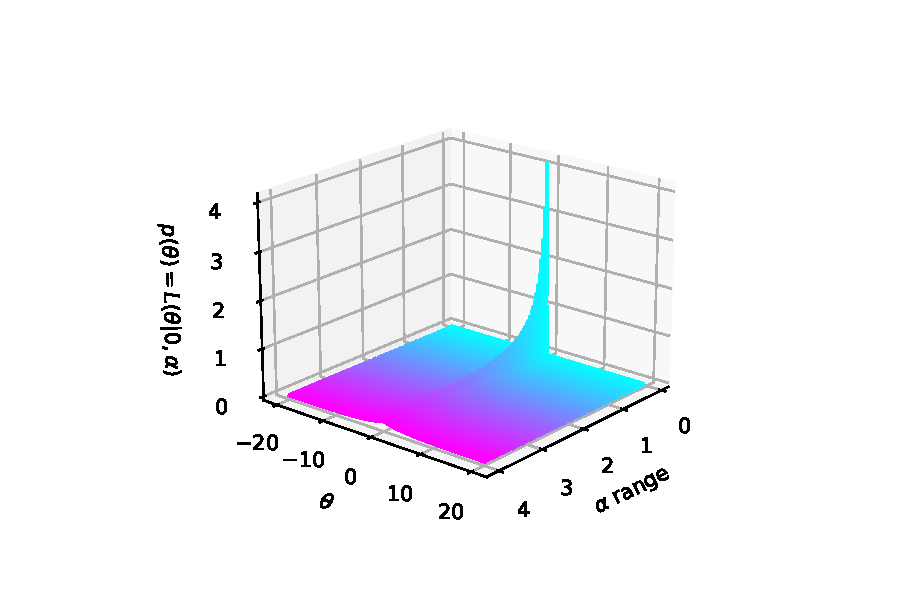
\includegraphics[width=\textwidth]{Q1a_8.pdf}
         \caption{$p(\theta \vert \alpha)$.}
     \end{subfigure}
     ~
     \begin{subfigure}[b]{0.45\textwidth}
         \centering
         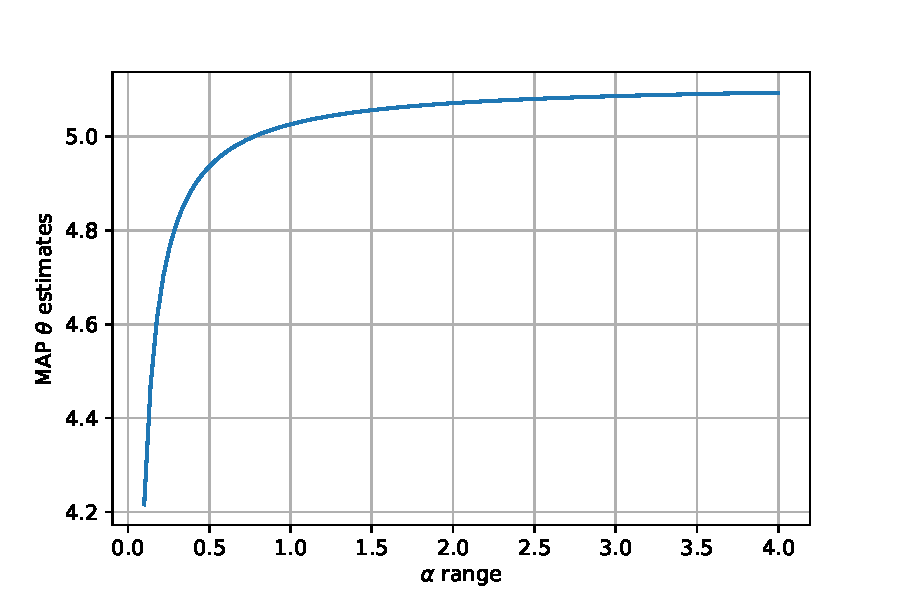
\includegraphics[width=\textwidth]{Q1a_9.pdf}
         \caption{MAP $\theta$ variation.}
     \end{subfigure}
     
     \begin{subfigure}[b]{0.45\textwidth}
         \centering
         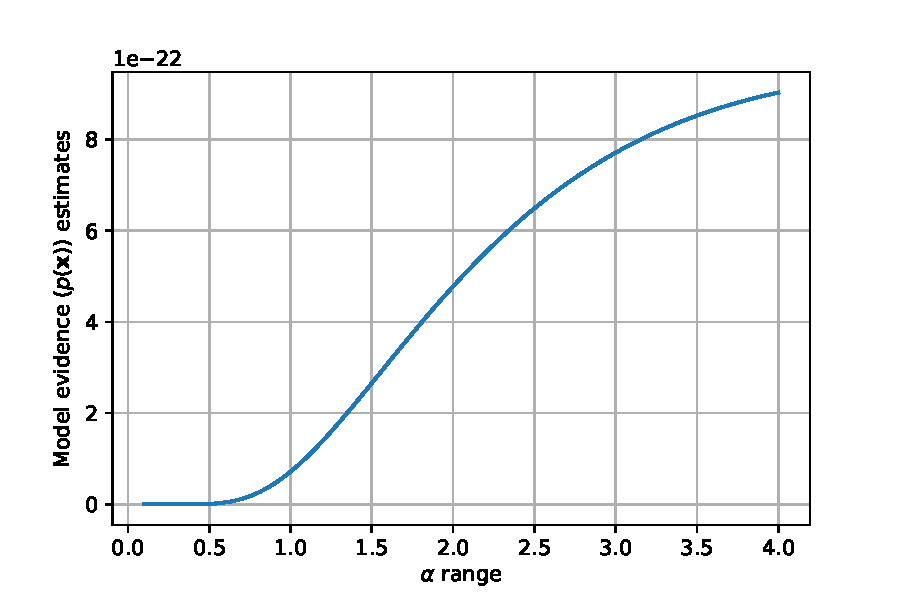
\includegraphics[width=\textwidth]{Q1a_10.pdf}
         \caption{Evidence $p(\mathbf{x})$ variation.}
     \end{subfigure}
     ~
     \begin{subfigure}[b]{0.45\textwidth}
         \centering
         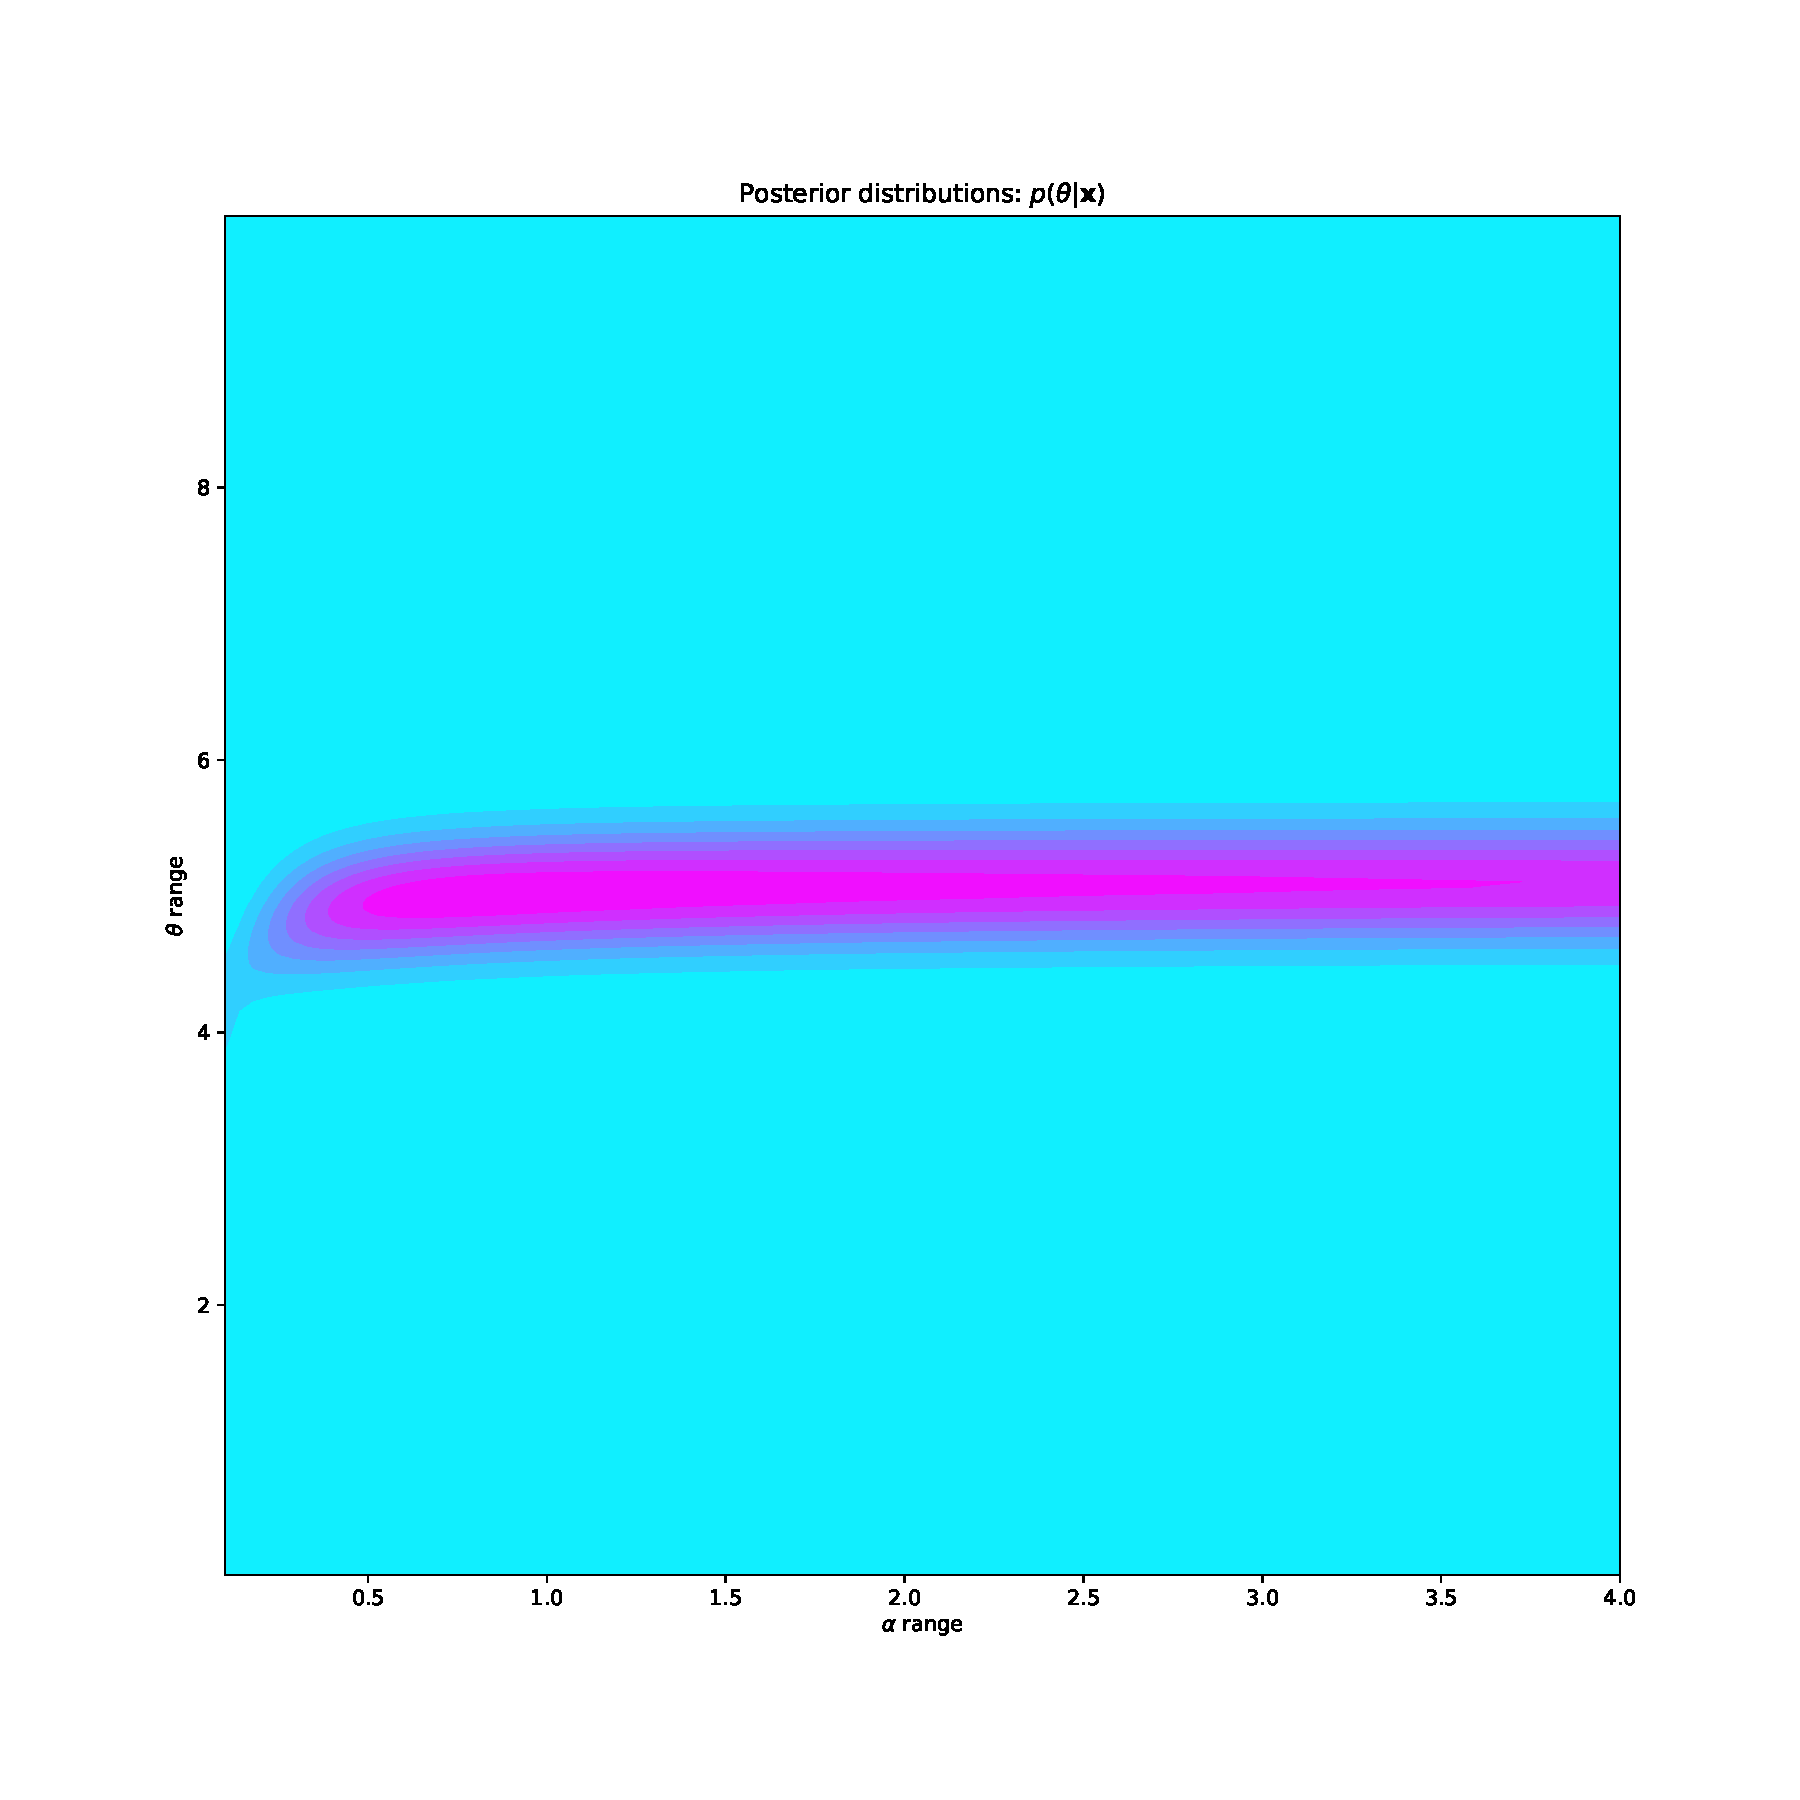
\includegraphics[width=\textwidth]{Q1a_12.pdf}
         \caption{Posterior $p(\theta \vert \mathbf{x})$ variation.}
     \end{subfigure}
     
     \caption{The influence of the prior variance $p(\theta \vert \alpha) = L(\theta \vert 0, \alpha)$ on the Bayesian inference process. In a) the prior is visualised over $\alpha$, in b) the variation of the MAP estimate for $\theta$ is shown, in c) the model evidence variation in shown, and in d) the variation of the posterior $p(\theta \vert \mathbf{x})$ is shown.}
     \label{fig:Q1a_alpha_variation}
\end{figure}


\subsection{Part B: Conjugate Bayesian inference}
asd

\iffalse

\begin{figure}[htb!]
\centering
\includegraphics[scale=0.5]{.pdf}
\caption{words words words.}
\label{fig:}
\end{figure}

\begin{figure}[htb!]
     \centering
     \begin{subfigure}[b]{0.45\textwidth}
         \centering
         \includegraphics[width=\textwidth]{.pdf}
         \caption{sub-words.}
     \end{subfigure}
     ~
     \begin{subfigure}[b]{0.45\textwidth}
         \centering
         \includegraphics[width=\textwidth]{.pdf}
         \caption{sub-words.}
     \end{subfigure}
     
     \caption{words words words.}
     \label{fig:}
\end{figure}

\fi

\clearpage

%Print the bibliography
\printbibliography

\end{document}
